\section{Overview}


simulations based on geant4 \cite{geant4} overview description, how geometry and digitization and calibration constants are loaded.

\subsection{Event Time Window}
\subsection{Hit Definition}
\subsection{True Information}
Process ID.

\subsection{Importing CAD volumes from the engineering model}


The Hall-B model is designed with 3D CAD software. This includes a reference system and the
hierarchy of all detector elements, down to details like nuts and bolts.


The CAD models are exported into STP files \cite{stepFiles}.
In order to import them into a geant4 simulation, first the volumes relevant to the simulation are selected, see \F{cadSelection}.

\begin{figure}
	\centering
	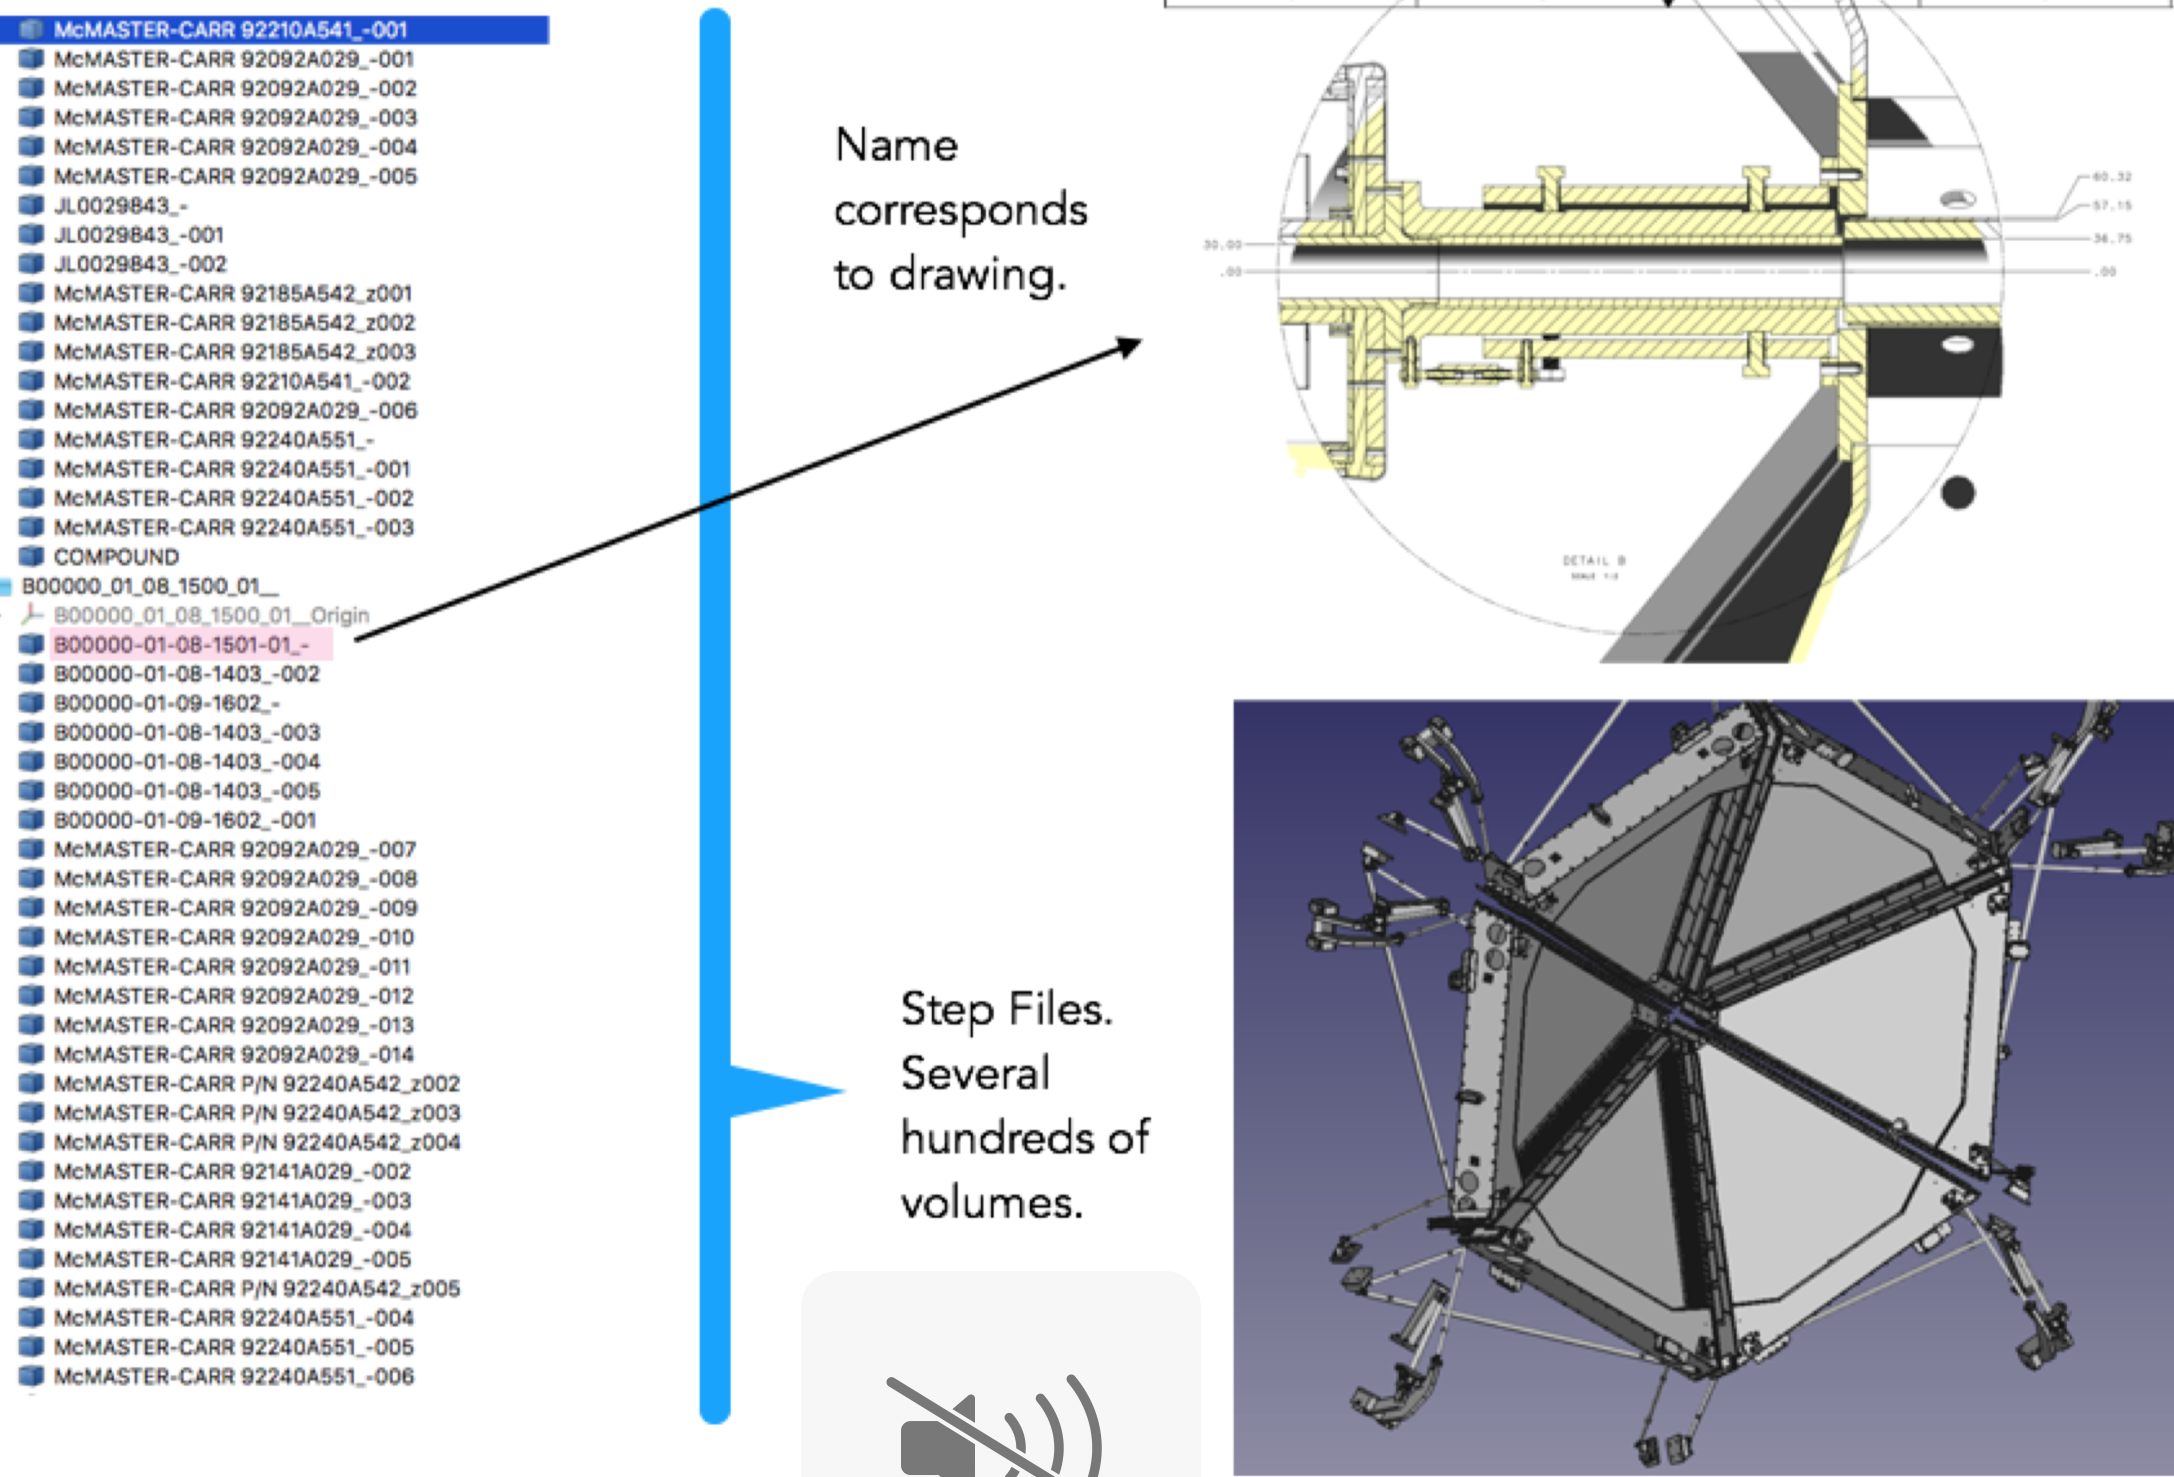
\includegraphics[width=0.98\columnwidth,keepaspectratio]{img/cadSelection.png}
	\caption{The selection of the volumes that will be used in the GEMC geant4 simulation.
             This typically involves filtering out unnecessary volumes that are not in the active region.}
	\label{fig:cadSelection}
\end{figure}


The elements in the STP file are then ``tessellated'': several polygon shapes are created to define a geant4 volume.
The software used to do this is FreeCad \cite{freeCad}. An example of tessellation showing the polygon shapes
is shown in \F{targetScatteringChamber}.

The simulated CAD import is as close to reality as the engineering model is close to reality.
We did encounter differences between the STP files, the drawings and reality in a few occasions and worked
out a workflow to eliminate any discrepancy, see \F{cadValidation}.


\begin{figure}
	\centering
	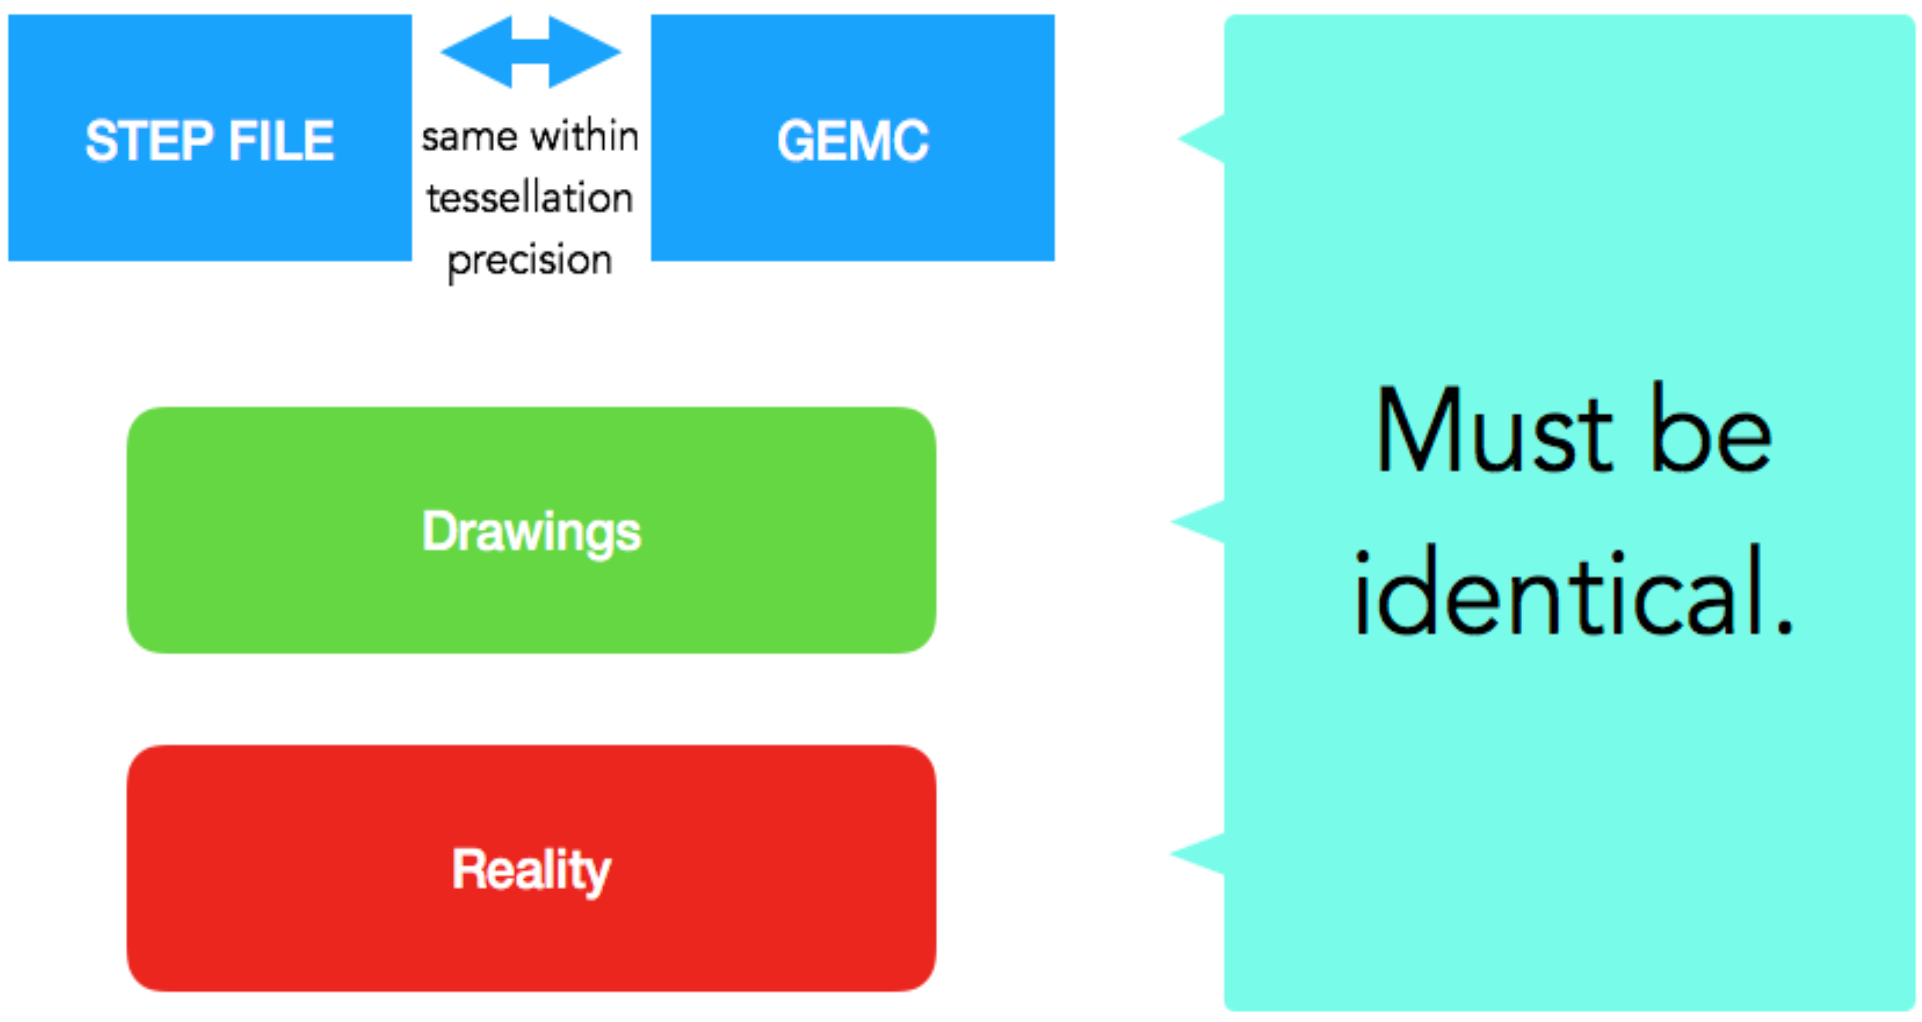
\includegraphics[width=0.95\columnwidth,keepaspectratio]{img/cadValidation.png}
	\caption{There are four possible representation of a volume: the one coming from the STP file
             and the tessellated one are exactly the same object (within the tessellation precision).
             In some cases, certain elements and their sizes and positions did not match the drawings.
             In other cases, they did not match what was built and measured, or their position did not
             match the survey. To eliminate these occurrences physicists and engineers worked until
             the final iteration of a volume was the same in all 4 models: STP/GEMC, Drawings and Reality}
	\label{fig:cadValidation}
\end{figure}

An example of the cad validation is shown in \F{cadValidationExample}.

\begin{figure}
	\centering
	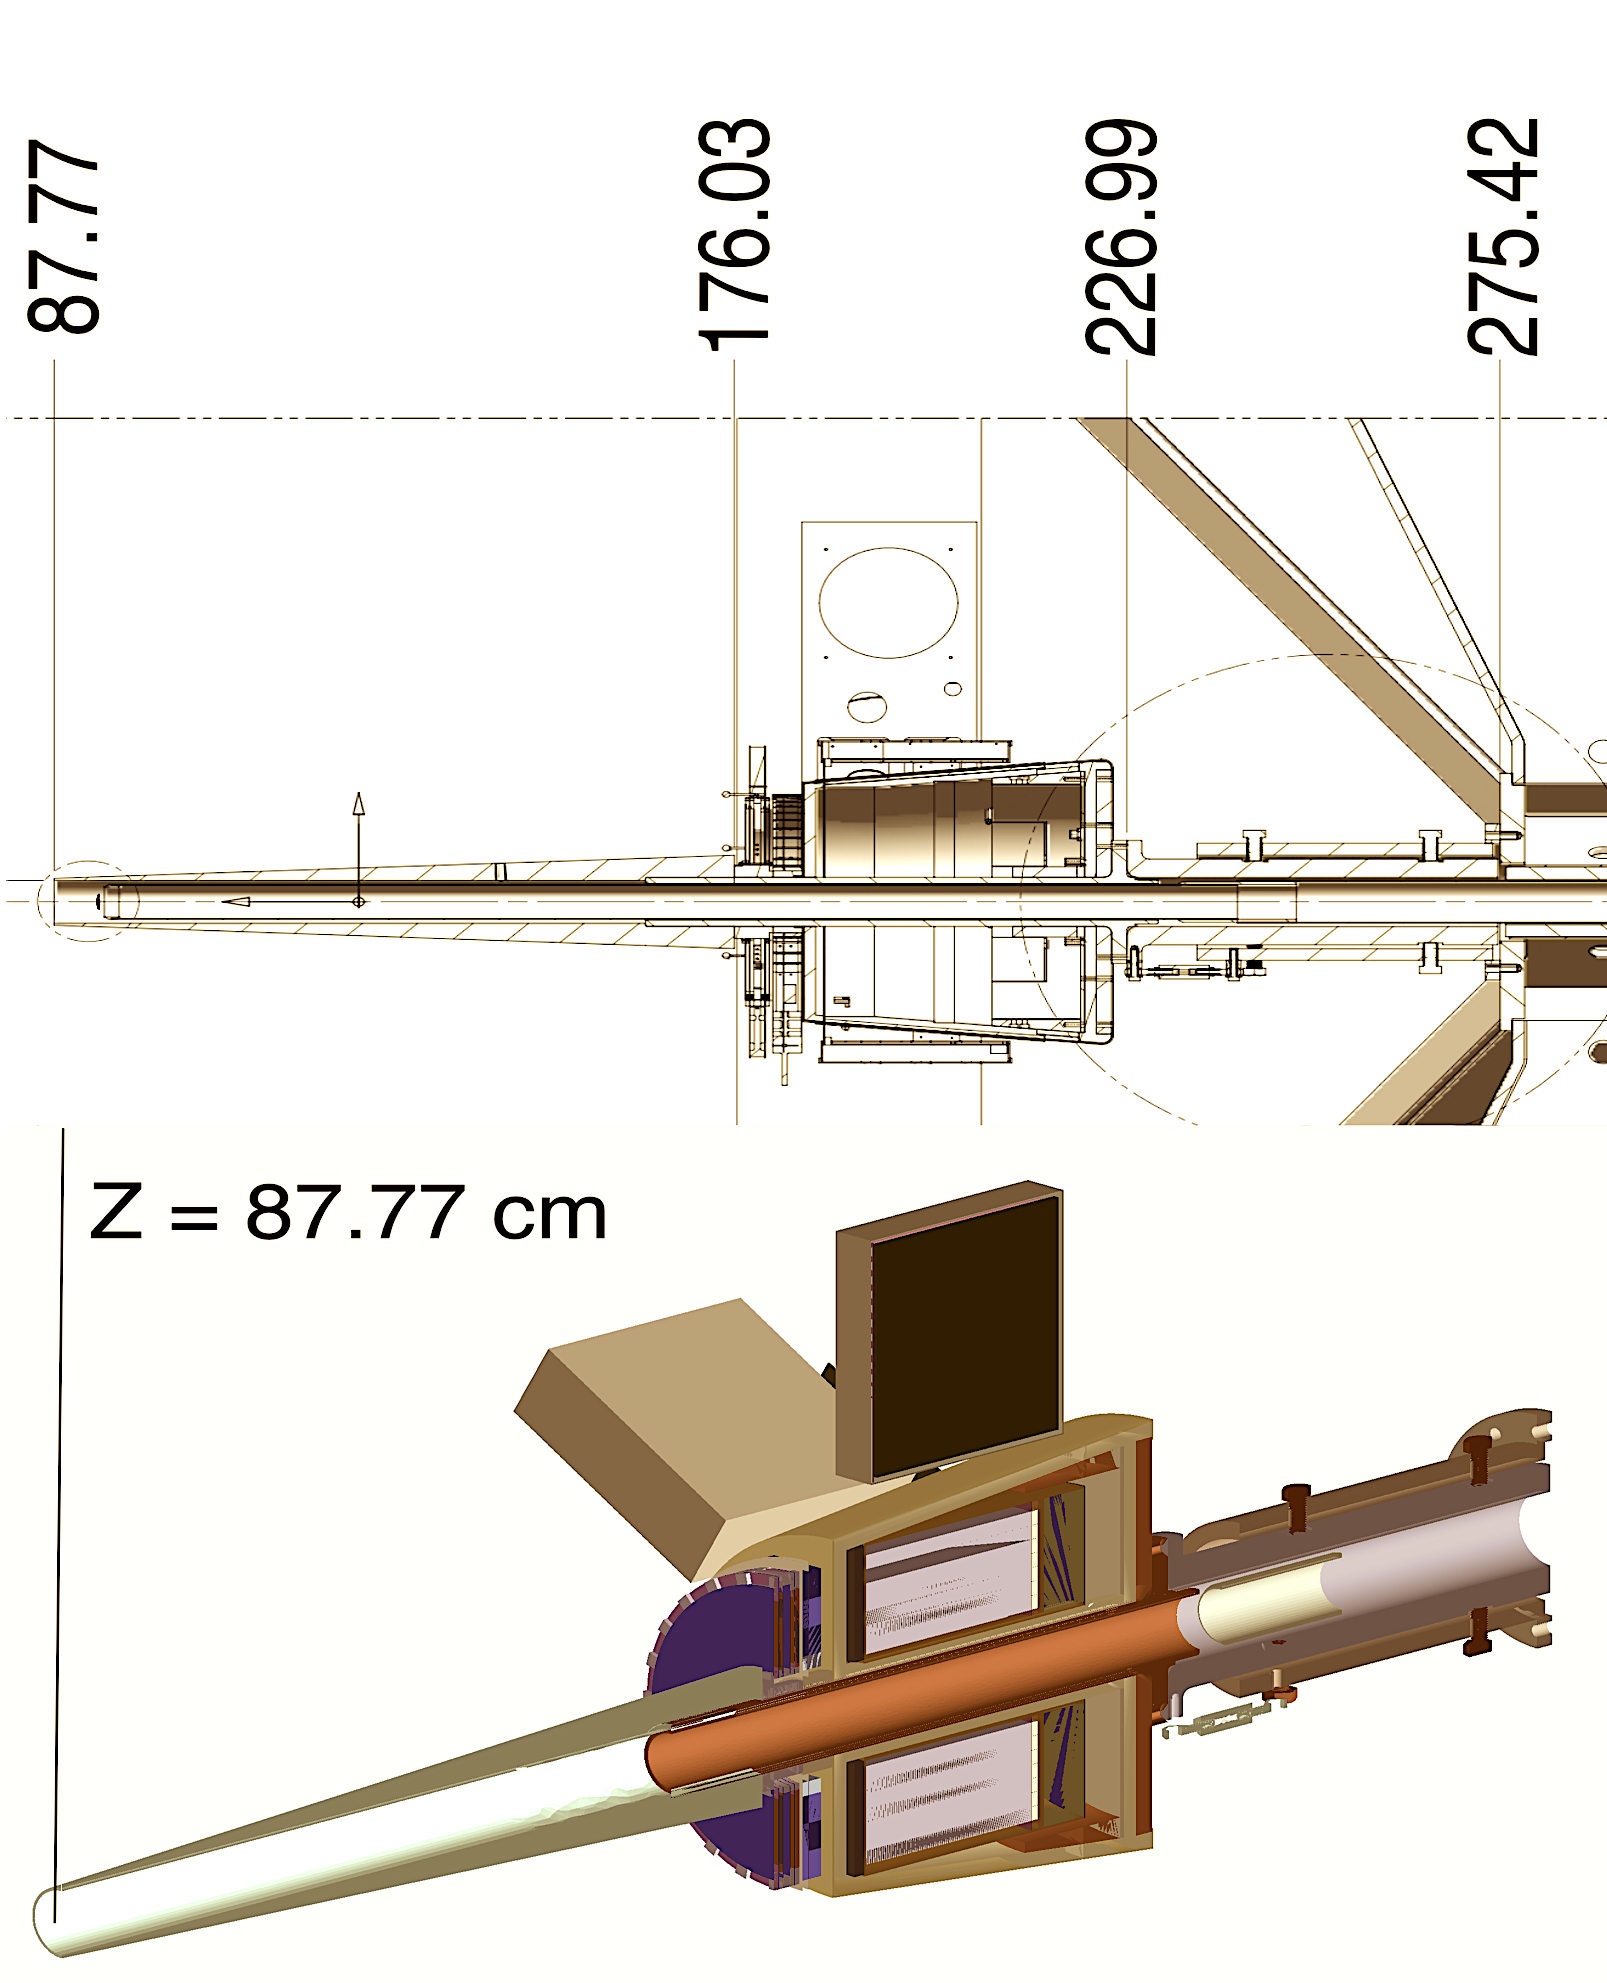
\includegraphics[width=0.95\columnwidth,keepaspectratio]{img/cadValidationExample.png}
	\caption{An example of comparing the gemc simulation to the drawings. Top: engineering drawings of
             the CLAS12 beamline and shielding. The start of the Moeller shielding is 87.77 cm downstream
             of the target center. Bottom: a geantino is shot vertically at z=87.77 cm, showing that the
             geant4 cone position agrees with the drawings.}
	\label{fig:cadValidationExample}
\end{figure}
